\section{Eigenvalue method with repeated eigenvalues}
\label{eigenmethod-repeat:section}

\LAtt{3.4, 3.7}

\LO{
\item Find generalized eigenvectors to write a general solution to a first order system with repeated and defective eigenvalues, and
\item Solve initial value problems from all of these cases once the general solution has been found. 
}

There is one remaining case for the two-component first-order linear system: repeated eigenvalues. As we have seen previously, it may happen that a matrix $A$ has some \myquote{repeated} eigenvalues.
That is, the characteristic equation $\det(A-\lambda I) = 0$ may have
repeated roots.  This is actually unlikely to happen
for a random matrix.  If we take a small perturbation of $A$ (we change the
entries of $A$ slightly), we get a matrix with distinct eigenvalues.  As
any system we want to solve in practice is an approximation to reality
anyway, it is not absolutely indispensable to know how to solve these
corner cases.  
On the other hand, these cases do come up in applications from time to time.
Furthermore, if we have distinct but very close eigenvalues, the behavior is
similar to that of repeated eigenvalues, and so understanding that case
will give us insight into what is going on.

\subsubsection{Geometric multiplicity}

Take the diagonal matrix
\begin{equation*}
A =
\begin{bmatrix}
3 & 0 \\ 0 & 3
\end{bmatrix} .
\end{equation*}
$A$ has an eigenvalue 3 of multiplicity 2.  We call the
multiplicity of the eigenvalue\index{multiplicity of an eigenvalue}
in the characteristic equation the
\emph{\myindex{algebraic multiplicity}}.  In this case, there also exist 2
linearly
independent eigenvectors,
$\left[ \begin{smallmatrix} 1 \\ 0 \end{smallmatrix} \right]$
and
$\left[ \begin{smallmatrix} 0 \\ 1 \end{smallmatrix} \right]$ corresponding
to the eigenvalue 3.  This means
that the so-called \emph{\myindex{geometric multiplicity}}
of this eigenvalue is also 2. These terms have all been discussed previously in \sectionref{eig:section}.

In all the
theorems where we required a matrix to have $n$ distinct eigenvalues, we only
really needed to have $n$ linearly independent eigenvectors.  For example,
${\vec{x}}' = A\vec{x}$ has the general solution
\begin{equation*}
\vec{x} = 
c_1 \begin{bmatrix} 1 \\ 0 \end{bmatrix} e^{3t}
+ c_2 \begin{bmatrix} 0 \\ 1 \end{bmatrix} e^{3t} .
\end{equation*}
Let us restate the theorem about real eigenvalues.  In the following theorem
we will repeat eigenvalues according to (algebraic) multiplicity.  So
for the matrix $A$ above, we would say that it has eigenvalues 3 and 3.

\begin{theorem1}{}
Suppose the $n \times n$ matrix $P$ 
has $n$ real eigenvalues (not necessarily distinct), $\lambda_1$,
$\lambda_2$, \ldots, $\lambda_n$,
and there are $n$ linearly independent corresponding eigenvectors
$\vec{v}_1$, $\vec{v}_2$, \ldots, $\vec{v}_n$.  Then the general solution to 
${\vec{x}}' = P\vec{x}$
can be written as
\begin{equation*}
\vec{x} = c_1 \vec{v}_1 e^{\lambda_1 t} +
c_2 \vec{v}_2 e^{\lambda_2 t} + \cdots +
c_n \vec{v}_n e^{\lambda_n t} .
\end{equation*}
\end{theorem1}
The main difference in the statement here from the theorem in \sectionref{eigenmethod:section} is that we are no longer assuming that we have $n$ \emph{distinct} eigenvalues. Instead, we need to assume that we end up with $n$ linearly independent eigenvectors, which we get for free if the eigenvalues are all distinct, but we might also have that if we do not have all distinct eigenvalues.

The \emph{geometric multiplicity} of an eigenvalue of algebraic multiplicity $n$
is equal to the number of corresponding linearly independent eigenvectors.
The geometric multiplicity is always less than or
equal to the algebraic multiplicity.  The theorem handles the case
when these two multiplicities are equal for all eigenvalues.
If for an eigenvalue the geometric multiplicity is equal
to the algebraic multiplicity, then we say the eigenvalue is
\emph{complete\index{complete eigenvalue}}.

In other words, 
the hypothesis of the theorem could be stated as saying that if all
the eigenvalues of $P$ are complete, then there are $n$ linearly independent
eigenvectors and thus we have the given general solution.

If the geometric multiplicity of an eigenvalue is 2 or greater,
then the set of linearly independent eigenvectors is not unique up to
multiples as it was before.  For example, for the diagonal matrix $A =
\left[ \begin{smallmatrix} 3 & 0 \\ 0 & 3 \end{smallmatrix} \right]$
we could also pick eigenvectors
$\left[ \begin{smallmatrix} 1 \\ 1 \end{smallmatrix} \right]$
and
$\left[ \begin{smallmatrix} 1 \\ -1 \end{smallmatrix} \right]$, or in fact
any pair of two linearly independent vectors.  The number of linearly
independent eigenvectors corresponding to $\lambda$
is the number of free variables we obtain when solving $A\vec{v} =
\lambda \vec{v}$.  We pick specific values for those free variables to
obtain eigenvectors.  If you pick different values, you may get different
eigenvectors.


\subsubsection{Defective eigenvalues}

If an $n \times n$ matrix has less than $n$ linearly independent
eigenvectors, it is said to be \emph{deficient\index{deficient matrix}}.
Then there is at least
one eigenvalue with an algebraic multiplicity that is higher than its geometric
multiplicity.  We call this eigenvalue \emph{defective\index{defective
eigenvalue}}
and the difference
between the two multiplicities we call the \emph{\myindex{defect}}.

\begin{example}
The matrix
\begin{equation*}
\begin{bmatrix}
3 & 1 \\ 0 & 3
\end{bmatrix}
\end{equation*}
has an eigenvalue 3 of algebraic multiplicity 2.
Let us try to compute eigenvectors.
\begin{equation*}
\begin{bmatrix}
0 & 1 \\ 0 & 0
\end{bmatrix}
\begin{bmatrix}
v_1 \\ v_2
\end{bmatrix}
= \vec{0} .
\end{equation*}
We must have that $v_2 = 0$.  Hence any eigenvector is of the form
$\left[ \begin{smallmatrix} v_1 \\ 0 \end{smallmatrix} \right]$.  Any two
such vectors are linearly dependent, and hence the geometric multiplicity
of the eigenvalue is 1.  Therefore, the defect is 1, and we can no longer
apply the eigenvalue method directly to a system of ODEs with such a
coefficient matrix.

\medskip

Roughly, the key observation is that
if $\lambda$ is an eigenvalue of $A$ of algebraic multiplicity $m$,
then we can find certain $m$ linearly independent vectors
solving ${(A-\lambda I)}^k \vec{v} = \vec{0}$ for various powers
$k$.  We will call these \emph{\myindex{generalized eigenvectors}}.

\medskip

Let us continue with the example
$A = \left[ \begin{smallmatrix}
3 & 1 \\ 0 & 3
\end{smallmatrix} \right]$ and the equation ${\vec{x}}' = A\vec{x}$.
We found an eigenvalue $\lambda=3$ of (algebraic) multiplicity 2 and defect 1.
We found one eigenvector 
$\vec{v} = \left[ \begin{smallmatrix} 1 \\ 0 \end{smallmatrix} \right]$.
We have one solution
\begin{equation*}
\vec{x}_1 = \vec{v} e^{3t} = \begin{bmatrix} 1 \\ 0 \end{bmatrix} e^{3t} .
\end{equation*}
We are now stuck, we get no other solutions from standard eigenvectors.  But
we need two linearly independent solutions to find the general solution of
the equation.

Let us try (in the spirit of repeated roots of the
characteristic equation for a single equation) another solution of the form
\begin{equation*}
\vec{x}_2 = \vec{v}_1 te^{3t},
\end{equation*}
since our modified guess for repeated roots from second order equations was $te^{3t}$. If we plug this guess into the equation, we get that
\begin{equation*}
\vec{x}_2' = \vec{v}_1 e^{3t} + 3\vec{v}_1te^{3t}
\end{equation*}
and since the right-hand side of the equation is $A\vec{v}_1te^{3t}$, we need $v_1$ to satisfy
\begin{equation*}
\vec{v}_1 e^{3t} + 3\vec{v}_1te^{3t} = A\vec{v}_1te^{3t}.
\end{equation*}
Since there is no $e^{3t}$ term on the right-hand side of the equation, we are forced to pick $\vec{v}_1 = \vec{0}$, and so  we get the solution $\vec{x}_2 = \vec{0}$, which is not good. This guess did not work.

The issue here is that we didn't have enough flexibility to actually get another solution to the differential equation, so we need something a little more complicated to make it work. To this end, we take a new guess of the form
\begin{equation*}
\vec{x}_2 = ( \vec{v}_2 +  \vec{v}_1 t )\, e^{3t} .
\end{equation*}
We differentiate to get
\begin{equation*}
{\vec{x}_2}' =
\vec{v}_1 e^{3t} +
3 ( \vec{v}_2 +  \vec{v}_1 t )\, e^{3t}
=
( 3 \vec{v}_2 + \vec{v}_1 )\, e^{3t} +  3 \vec{v}_1 t e^{3t} .
\end{equation*}
As we are assuming that $\vec{x}_2$ is a solution, ${\vec{x}_2}'$ must
equal $A \vec{x}_2$. So let's compute $A \vec{x}_2$:
\begin{equation*}
A \vec{x}_2 = 
A ( \vec{v}_2 +  \vec{v}_1 t )\, e^{3t}
=
A \vec{v}_2 e^{3t} +  A \vec{v}_1 t e^{3t} .
\end{equation*}
By looking at the coefficients of $e^{3t}$ and $t e^{3t}$ we see
$3 \vec{v}_2 + \vec{v}_1 = A \vec{v}_2$ and
$3 \vec{v}_1 = A \vec{v}_1$.
This means that
\begin{equation*}
(A-3I)\vec{v}_2 = \vec{v}_1,
\qquad \text{and} \qquad
(A-3I)\vec{v}_1 = \vec{0}.
\end{equation*}
Therefore, $\vec{x}_2$ is a solution
if these two equations are satisfied.
The second equation is satisfied if $\vec{v}_1$ is an
eigenvector, and we found the eigenvector above, so let
$\vec{v}_1 = 
\left[ \begin{smallmatrix} 1 \\ 0 \end{smallmatrix} \right]$.
So, if we can find a $\vec{v}_2$ that solves
%${(A-3I)}^2\vec{v}_2 = \vec{0}$ and such that
$(A-3I)\vec{v}_2 = \vec{v}_1$, then we are done.
This is just a bunch of linear
equations to solve and we are by now very good at that.
%
Let us solve
$(A-3I)\vec{v}_2 = \vec{v}_1$.  Write
\begin{equation*}
\begin{bmatrix}
0 & 1 \\ 0 & 0
\end{bmatrix}
\begin{bmatrix}
a \\ b
\end{bmatrix}
=
\begin{bmatrix}
1 \\ 0
\end{bmatrix} .
\end{equation*}
By inspection we see that letting $a=0$ ($a$ could be anything in fact) and
$b=1$ does the job.  Hence we can take $\vec{v}_2 = 
\left[ \begin{smallmatrix} 0 \\ 1 \end{smallmatrix} \right]$.  Our general
solution to
${\vec{x}}' = A\vec{x}$ is
\begin{equation*}
\vec{x} =
c_1 
\begin{bmatrix}
1 \\ 0
\end{bmatrix}
e^{3t}
+
c_2
\left(
\begin{bmatrix}
0 \\ 1
\end{bmatrix}
+
\begin{bmatrix}
1 \\ 0
\end{bmatrix}
t
\right)
\,
e^{3t}
=
\begin{bmatrix}
c_1 e^{3t}+c_2 te^{3t} \\
c_2 e^{3t}
\end{bmatrix} .
\end{equation*}
Let us check that we really do have the solution.  First
$x_1' = 
c_1 3 e^{3t}+c_2 e^{3t} + 3 c_2 te^{3t} = 3 x_1 + x_2$.  Good.  Now
$x_2' = 3 c_2 e^{3t} = 3x_2$.  Good.
\end{example}

In the example, if we plug $(A-3I)\vec{v}_2 = \vec{v}_1$ into
$(A-3I)\vec{v}_1 = \vec{0}$ we find
\begin{equation*}
(A-3I)(A-3I) \vec{v}_2 = \vec{0},
\qquad \text{or} \qquad
{(A-3I)}^2\vec{v}_2 = \vec{0}.
\end{equation*}
Furthermore, if 
$(A-3I) \vec{w} \not= \vec{0}$, then 
$(A-3I) \vec{w}$ is an eigenvector, a multiple of $\vec{v}_1$.
In this $2 \times 2$ case ${(A-3I)}^2$ is just the zero matrix (exercise).
So any vector $\vec{w}$ solves
${(A-3I)}^2\vec{w} = \vec{0}$ and we just need a $\vec{w}$ such that
$(A-3I)\vec{w} \not= \vec{0}$.  Then we could use
$\vec{w}$ for $\vec{v}_2$, and $(A-3I)\vec{w}$ for $\vec{v}_1$.

Note that the system ${\vec{x}}' = A \vec{x}$ has a simpler solution since
$A$ is a so-called \emph{\myindex{upper triangular matrix}}, that is
every entry below the diagonal is zero.
In particular, the equation for $x_2$
does not depend on $x_1$.  Mind you, not every defective matrix is
triangular.

\begin{exercise}
Solve ${\vec{x}}' = \left[ \begin{smallmatrix}
3 & 1 \\ 0 & 3
\end{smallmatrix} \right] \vec{x}$ by first solving for $x_2$ and then for
$x_1$ independently.  Check that you got the same solution as we did
above.
\end{exercise}

Let us describe the general algorithm.  Suppose that $\lambda$ is an
eigenvalue of multiplicity 2, defect 1.
First find an eigenvector $\vec{v}_1$ of $\lambda$.  
That is, $\vec{v}_1$ solves
$(A-\lambda I)\vec{v}_1  = \vec{0}$.
Then, find a vector $\vec{v}_2$ such that
\begin{equation*}
%{(A-\lambda I)}^2\vec{v}_2 & = \vec{0} , \\
(A-\lambda I)\vec{v}_2 = \vec{v}_1 .
\end{equation*}
This gives us two linearly independent solutions
\begin{align*}
\vec{x}_1 & = \vec{v}_1 e^{\lambda t} , \\
\vec{x}_2 & = \left( \vec{v}_2 + \vec{v}_1 t \right) e^{\lambda t},
\end{align*}
and so our general solution to the differential equation is
\begin{equation*}
\vec{x}(t) = c_1\vec{v}_1e^{\lambda t} + c_2\left(\vec{v}_2 + \vec{v}_1 t \right) e^{\lambda t}.
\end{equation*}

\begin{example}
Solve the initial value problem
\begin{equation*}
\vec{x}' = \begin{bmatrix} -2 & 3 \\ -3 & 4 \end{bmatrix}\vec{x} \qquad \vec{x}(0) = \begin{bmatrix} 2 \\ -1 \end{bmatrix}.
\end{equation*}
\end{example}

\begin{exampleSol}
First, we need to look for the eigenvalues of the coefficient matrix. These are found by
\begin{equation*}
\det(A - \lambda I) = (-2-\lambda)(4-\lambda) - (3)(-3) = \lambda^2 - 2\lambda + 1 = 0.
\end{equation*}
Since this polynomial is $(\lambda - 1)^2$, this has a double root at $\lambda = 1$. 

For $\lambda = 1$, we can hunt for the eigenvector as solutions to
\begin{equation*}
(A - I)\vec{v} = \begin{bmatrix} -3 & 3 \\ -3 & 3 \end{bmatrix} \vec{v} = 0.
\end{equation*}
These two equations are redundant, and the first equation is $-3v_1 + 3v_2 = 0$, which can be solved by $v_1 = v_2 = 1$. Therefore, and an eigenvector for $\lambda = 1$ is $\left[ \begin{smallmatrix} 1 \\ 1 \end{smallmatrix} \right]$. Thus, we have a solution to this system of the form
\begin{equation*}
\vec{x}_1(t) = \begin{bmatrix} 1 \\ 1 \end{bmatrix} e^t.
\end{equation*}

Since we only found one eigenvector, we need to look for a generalized eigenvector as well. To do this, we want to solve the equation
\begin{equation*}
(A - I)\vec{w} = \vec{v}
\end{equation*} 
for the eigenvector $\vec{v}$ that we found previously. This means we need to solve
\begin{equation*}
\begin{bmatrix} -3 & 3 \\ -3 & 3 \end{bmatrix} \vec{w} = \begin{bmatrix} 1 \\ 1 \end{bmatrix}
\end{equation*}
and both rows of the vector equation result in the equation $-3w_1 + 3w_2 = 1$ for $\vec{w}$. We can pick \emph{any} value of $w_1$ and $w_2$ to make this work. For the sake of this example, we will pick $w_1 = 0$ and $w_2 = \nicefrac{1}{3}$. Then, we have that our second linearly independent solution to the differential equation is
\begin{equation*}
\vec{x}_2(t) = \left(\begin{bmatrix} 0 \\ 1/3 \end{bmatrix} + \begin{bmatrix} 1 \\ 1 \end{bmatrix} t \right) e^{t}
\end{equation*}
and so the general solution to this system is
\begin{equation*}
\vec{x}(t) = c_1 \begin{bmatrix} 1 \\ 1 \end{bmatrix} e^t + c_2 \left(\begin{bmatrix} 0 \\ 1/3 \end{bmatrix} + \begin{bmatrix} 1 \\ 1 \end{bmatrix} t \right) e^{t}.
\end{equation*}

Finally, we can solve the initial value problem. Plugging in $t=0$ gives
\begin{equation*}
\vec{x}(0) = c_1 \begin{bmatrix} 1 \\ 1 \end{bmatrix} + c_2 \begin{bmatrix} 0 \\ 1/3 \end{bmatrix} = \begin{bmatrix} 2 \\ -1 \end{bmatrix},
\end{equation*}
which gives that $c_1 = 2$ and then $2 + \nicefrac{1}{3}c_2 = -1$, or $c_2 = -9$. Therefore, the solution to the initial value problem is
\begin{equation*}
\vec{x}(t) = 2 \begin{bmatrix} 1 \\ 1 \end{bmatrix} e^t - 9 \left(\begin{bmatrix} 0 \\ 1/3 \end{bmatrix} + \begin{bmatrix} 1 \\ 1 \end{bmatrix} t \right) e^{t}.
\end{equation*}
\end{exampleSol}

\begin{exercise}
We could have also chosen $w_1 = -\nicefrac{1}{3}$ and $w_2 = 0$ for the vector $\vec{w}$. Use this to get a different looking general solution. Then solve the same initial value problem to see that you end up with the same answer at the end of the process. 
\end{exercise}

\begin{example}
Consider the system
\begin{equation*}
\vec{x}' =
\begin{bmatrix}
2 & -5 & 0 \\
0 & 2 & 0 \\
-1 & 4 & 1
\end{bmatrix}
\vec{x} .
\end{equation*}
Find the general solution to this system using eigenvalues and eigenvectors.
\end{example}

\begin{exampleSol}
Even though this is a three-component system, the process is exactly the same: find the eigenvalues, compute corresponding eigenvectors, then build them together into a general solution. Compute the eigenvalues,
\begin{equation*}
0 =
\det(A-\lambda I) = 
\det\left(
\begin{bmatrix}
2-\lambda & -5 & 0 \\
0 & 2-\lambda & 0 \\
-1 & 4 & 1-\lambda
\end{bmatrix}
\right)
= (2-\lambda)^2(1-\lambda) .
\end{equation*}
The eigenvalues are 1 and 2, where 2 has multiplicity 2.
We leave it to the reader to find that
$\left[ \begin{smallmatrix} 0 \\ 0 \\ 1 \end{smallmatrix} \right]$
is an eigenvector
for the eigenvalue $\lambda = 1$.

Let's focus on $\lambda = 2$.  We compute eigenvectors:
\begin{equation*}
\vec{0} =
(A - 2 I) \vec{v}
=
\begin{bmatrix}
0 & -5 & 0 \\
0 & 0 & 0 \\
-1 & 4 & -1
\end{bmatrix}
\begin{bmatrix}
v_1 \\ v_2 \\ v_3
\end{bmatrix}
.
\end{equation*}
The first equation says that $v_2 = 0$, so the last equation
is $-v_1 -v_3 = 0$.  Let $v_3$ be the free variable to find
that $v_1 = -v_3$.  Perhaps let $v_3 = -1$ to find an eigenvector
$\left[ \begin{smallmatrix} 1 \\ 0 \\ -1 \end{smallmatrix} \right]$.
Problem is that setting $v_3$ to anything else just gets multiples
of this vector and so we have a defect of 1.
Let $\vec{v}_1$ be the eigenvector and let's look for
a generalized eigenvector $\vec{v}_2$:
\begin{equation*}
(A - 2 I) \vec{v}_2 = \vec{v}_1 , 
\end{equation*}
or
\begin{equation*}
\begin{bmatrix}
0 & -5 & 0 \\
0 & 0 & 0 \\
-1 & 4 & -1
\end{bmatrix}
\begin{bmatrix}
a \\ b \\ c
\end{bmatrix}
=
\begin{bmatrix}
1 \\ 0 \\ -1
\end{bmatrix} ,
\end{equation*}
where we used $a$, $b$, $c$ as components of $\vec{v}_2$ for simplicity.
The first equation says $-5b = 1$ so $b = \nicefrac{-1}{5}$.  The
second equation says nothing.
The last equation is $-a + 4b - c = -1$, or
$a + \nicefrac{4}{5} + c = 1$, or
$a + c = \nicefrac{1}{5}$.  We let $c$ be the free variable and we
choose $c=0$.  We find
$\vec{v}_2 = \left[ \begin{smallmatrix} \nicefrac{1}{5} \\ \nicefrac{-1}{5}
\\ 0 \end{smallmatrix} \right]$.

The general solution is therefore,
\begin{equation*}
\vec{x} =
c_1
\begin{bmatrix} 0 \\ 0 \\ 1 \end{bmatrix}
e^t
+
c_2 
\begin{bmatrix} 1 \\ 0 \\ -1 \end{bmatrix}
e^{2t}
+
c_3
\left(
\begin{bmatrix} \nicefrac{1}{5} \\ \nicefrac{-1}{5} \\ 0 \end{bmatrix}
+
\begin{bmatrix} 1 \\ 0 \\ -1 \end{bmatrix}
t
\right)
e^{2t}
.
\end{equation*}
\end{exampleSol}

This machinery can also be generalized to higher multiplicities
and higher defects.
We will not go over this method in detail, but let us just sketch the ideas.  Suppose that $A$
has an eigenvalue $\lambda$ of multiplicity $m$.
We find vectors such that
\begin{equation*}
{(A - \lambda I)}^k \vec{v}_k = \vec{0},
\qquad \text{but} \qquad
{(A - \lambda I)}^{k-1} \vec{v}_k \not= \vec{0}.
\end{equation*}
Such vectors are called \emph{\myindex{generalized eigenvectors}} (then
$\vec{v}_1 = {(A - \lambda I)}^{k-1} \vec{v}_k$ is an eigenvector).
For the
eigenvector $\vec{v}_1$ there is a chain of generalized eigenvectors
$\vec{v}_2$ through $\vec{v}_k$ such that:
\begin{align*}
(A - \lambda I) \vec{v}_1 & = \vec{0} , \\
(A - \lambda I) \vec{v}_2 & = \vec{v}_1 , \\
& ~~\vdots \\
(A - \lambda I) \vec{v}_k & = \vec{v}_{k-1} .
\end{align*}
Really once you find the $\vec{v}_k$ such that
${(A - \lambda I)}^k \vec{v}_k = \vec{0}$ but
${(A - \lambda I)}^{k-1} \vec{v}_k \not= \vec{0}$, you find the entire
chain since you can compute the rest,
$\vec{v}_{k-1} = (A - \lambda I) \vec{v}_k$,
$\vec{v}_{k-2} = (A - \lambda I) \vec{v}_{k-1}$, etc.
We form the linearly independent solutions
\begin{align*}
\vec{x}_1 & = \vec{v}_1 e^{\lambda t} , \\
\vec{x}_2 & = ( \vec{v}_2 + \vec{v}_1 t ) \, e^{\lambda t} , \\
& ~~\vdots \\
\vec{x}_k & = \left( \vec{v}_k + \vec{v}_{k-1} t +
\vec{v}_{k-2} \frac{t^2}{2} +
\cdots + \vec{v}_2 \frac{t^{k-2}}{(k-2)!} + \vec{v}_1 \frac{t^{k-1}}{(k-1)!}
\right) \, e^{\lambda t} .
\end{align*}
Recall that $k! = 1 \cdot 2 \cdot 3 \cdots (k-1) \cdot k$ is the factorial.
If you have an eigenvalue of geometric multiplicity $\ell$,
you will have to find $\ell$ such chains (some of them might be
short: just the single eigenvector equation).
We go until we form $m$ linearly independent solutions where
$m$ is the algebraic multiplicity.
We don't quite know which specific eigenvectors go with which chain, so
start by finding $\vec{v}_k$ first for the longest possible chain and
go from there.

For example, if $\lambda$ is an eigenvalue of $A$
of algebraic multiplicity 3 and defect 2, then solve
\begin{equation*}
(A - \lambda I) \vec{v}_1 = \vec{0} , \qquad
(A - \lambda I) \vec{v}_2 = \vec{v}_1 , \qquad
(A - \lambda I) \vec{v}_3 = \vec{v}_2 .
\end{equation*}
That is, find $\vec{v}_3$ such that 
${(A - \lambda I)}^3 \vec{v}_3 = \vec{0}$, but
${(A - \lambda I)}^2 \vec{v}_3 \not= \vec{0}$.
Then you are done as
$\vec{v}_2 = (A - \lambda I) \vec{v}_3$
and 
$\vec{v}_1 = (A - \lambda I) \vec{v}_2$.
The 3 linearly independent solutions are
\begin{equation*}
\vec{x}_1 = \vec{v}_1 e^{\lambda t} , \qquad
\vec{x}_2 = ( \vec{v}_2 + \vec{v}_1 t ) \, e^{\lambda t} , \qquad
\vec{x}_3 = \left( \vec{v}_3 + \vec{v}_2 t +
\vec{v}_{1} \frac{t^2}{2} \right) \, e^{\lambda t} .
\end{equation*}

If on the other hand $A$ has an eigenvalue $\lambda$
of algebraic multiplicity 3 and defect 1, then 
solve
\begin{equation*}
(A - \lambda I) \vec{v}_1 = \vec{0} , \qquad
(A - \lambda I) \vec{v}_2 = \vec{0} , \qquad
(A - \lambda I) \vec{v}_3 = \vec{v}_2 .
\end{equation*}
Here $\vec{v}_1$ and $\vec{v}_2$ are actual honest eigenvectors,
and $\vec{v}_3$ is a generalized eigenvector.
So there are two chains.
To solve, first find a 
$\vec{v}_3$ such that 
${(A - \lambda I)}^2 \vec{v}_3 = \vec{0}$, but
$(A - \lambda I) \vec{v}_3 \not= \vec{0}$.
Then $\vec{v}_2 = (A - \lambda I) \vec{v}_3$ is going to be an eigenvector.
Then solve for an eigenvector $\vec{v}_1$ that is linearly independent 
from $\vec{v}_2$.
You get 3 linearly independent solutions
\begin{equation*}
\vec{x}_1 = \vec{v}_1 e^{\lambda t} , \qquad
\vec{x}_2 = \vec{v}_2 e^{\lambda t} , \qquad
\vec{x}_3 = ( \vec{v}_3 + \vec{v}_2 t ) \, e^{\lambda t} .
\end{equation*}

\subsection{Phase Portraits}

We also want to look at the phase portraits and direction field diagrams for repeated eigenvalues. There are two different options here, depending on if there are two linearly independent eigenvectors or not.

\emph{Case 1.} If we have a repeated eigenvalue with two linearly independent eigenvectors, this means that our matrix $A$ is of the form
\[ A = \begin{bmatrix} \lambda & 0 \\ 0 & \lambda \end{bmatrix} \] for the repeated eigenvalue $\lambda$. This means that $A \vec{v} = \lambda \vec{v}$ for all vectors $\vec{v}$. So, every vector is part of a straight line solution, and so every solution goes either directly towards or directly away from the origin. This gives a \emph{\myindex{proper node}} which can be a sink or a source depending on whether the eigenvalue is positive or negative. 

\begin{myfig}
\capstart
\myincludegraphics{width=2.8in}{width=4in}{pln-proper-sinkfig}
\caption{Example proper nodal sink vector field.\label{pln:proper-sinkfig}}
\end{myfig}

\emph{Case 2.} If we have a repeated eigenvalue with only one linearly independent eigenvector, then we only have one straight-line solution. For instance, the matrix 
\[ A = \begin{bmatrix} 4 & -1 \\ 1 & 2 \end{bmatrix} \] has only one eigenvector of $\begin{bmatrix} 1 \\ 1 \end{bmatrix}$ for eigenvalue $3$. Like the nodal sources and sinks, the solutions will go to zero and infinity along the straight line solutions. In this case, because there is only one straight line, the phase portrait looks somewhere between a node and a spiral. This gives an \emph{\myindex{improper node}} which can be a source or sink depending on the sign of the eigenvalue.

\begin{myfig}
\capstart
\myincludegraphics{width=3in}{width=4.5in}{pln-improper-sourcefig}
\caption{Example improper nodal source vector field.\label{pln:improper-sourcefig}}
\end{myfig}

\subsection{Exercises}

%Repeated eigenvalue, do not ask to solve a diffy q quite yet
\begin{exercise}
Compute eigenvalues and eigenvectors of
$\left[ \begin{smallmatrix}
-2 & -1 & -1 \\
3 & 2 & 1 \\
-3 & -1 & 0 \\
\end{smallmatrix} \right]$.
\end{exercise}
\comboSol{%
}
{%
$\lambda_1 = -2$, $\vec{v}_1 = \left[\begin{smallmatrix} -1 \\ 1 \\ -1 \end{smallmatrix}\right]$. $\lambda_2 = 1$, two-dimensional space of eigenvectors, options: $\left\{ \left[\begin{smallmatrix} -1 \\ 0 \\ 3 \end{smallmatrix}\right],\ \left[\begin{smallmatrix} -1 \\ 3 \\ 0 \end{smallmatrix}\right]\right\}$
}

\begin{exercise}
Let
$A = \left[ \begin{smallmatrix} 5 & -3 \\ 3 & -1 \end{smallmatrix} \right]$.
Find the general solution of ${\vec{x}}' = A \vec{x}$ and sketch the corresponding phase portrait.
\end{exercise}
\comboSol{%
}
{%
$\vec{x}(t) = C_1 \left[\begin{smallmatrix}  1\\ 1 \end{smallmatrix}\right]e^{2t} + C_2\left( \left[\begin{smallmatrix} 1\\1 \end{smallmatrix}\right]te^{2t} + \left[\begin{smallmatrix} 1/3 \\ 0 \end{smallmatrix}\right]e^{2t}\right)$ \hfill\raisebox{-0.5\height}{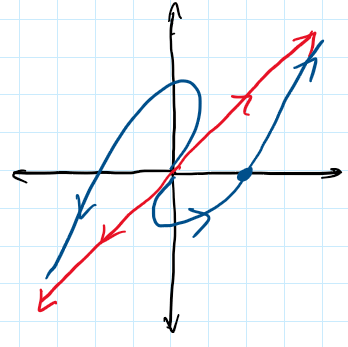
\includegraphics[height=1.5in]{Images/phaseportrait_5_n3_3_n1_sketch.png}}\hfill\hfill
}

\begin{exercise}
Solve the initial value problem
\[ {\vec{x}}' = \begin{bmatrix} -3 & 2 \\ 0 & -3 \end{bmatrix} \vec{x} \qquad \vec{x}(0) = \begin{bmatrix} 2 \\ 1 \end{bmatrix} \] and sketch the phase portrait for this system.
\end{exercise}
\comboSol{%
}
{%
$\vec{x}(t) = \left[\begin{smallmatrix} (2t+2)e^{-3t} \\ (2t+1)e^{-3t} \end{smallmatrix}\right]$ \hfill\raisebox{-0.5\height}{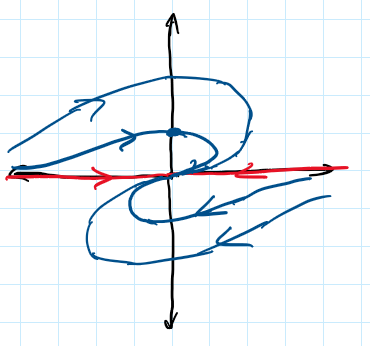
\includegraphics[height=1.5in]{Images/phaseportrait_n3_2_0_n3_sketch.png}}\hfill\hfill
}


\begin{exercise}
Solve the initial value problem
\[ {\vec{x}}' = \begin{bmatrix} -5 & -2 \\ 8 & 3 \end{bmatrix} \vec{x} \qquad \vec{x}(0) = \begin{bmatrix} 1 \\ 1 \end{bmatrix} \] and sketch the phase portrait for this system.
\end{exercise}
\comboSol{%
}
{%
$\vec{x}(t) = \left[\begin{smallmatrix} (-6t+1)e^{-t} \\ (12t+1)e^{-t} \end{smallmatrix}\right]$ \hfill\raisebox{-0.5\height}{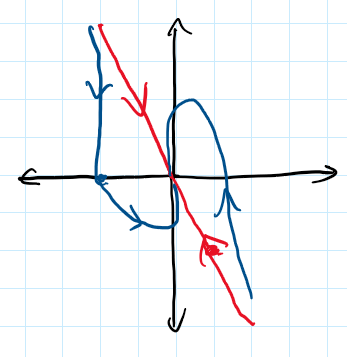
\includegraphics[height=1.5in]{Images/phaseportrait_n5_n2_8_3_sketch.png}}\hfill\hfill
}

\begin{exercise}
Solve the initial value problem
\[ {\vec{x}}' = \begin{bmatrix} -3 & -12 \\ 3 & 9 \end{bmatrix}\vec{x} \qquad \vec{x}(0) = \begin{bmatrix} 3 \\ 2  \end{bmatrix} \] and sketch the phase portrait for this system.
\end{exercise}
\comboSol{%
}
{%
$\vec{x}(t) = \left[\begin{smallmatrix} (-42t+3)e^{3t} \\ (21t + 2)e^{3t} \end{smallmatrix}\right]$ \hfill\raisebox{-0.5\height}{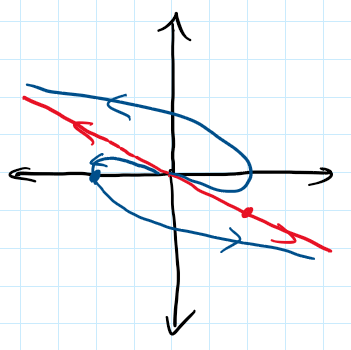
\includegraphics[height=1.5in]{Images/phaseportrait_n3_n12_3_9_sketch.png}}\hfill\hfill
}

\begin{exercise}
Assume $A$ is a $3\times 3$ matrix. The row-reduced echelon forms of $A-\lambda I$ are given for three different values of $\lambda$:
$$A-3I \rightsquigarrow \begin{pmatrix} 1&0&0\\ 0&1&0\\ 0&0&1 \end{pmatrix} \qquad\qquad 
A-5I \rightsquigarrow \begin{pmatrix} 1&4&0\\ 0&0&1\\ 0&0&0 \end{pmatrix}\qquad\qquad
A-7I \rightsquigarrow \begin{pmatrix} 1&-1&1/2\\ 0&0&0\\ 0&0&0 \end{pmatrix}$$

Find the general solution of the homogeneous system $\vec{x}'=A\vec{x}$.
\end{exercise}
\comboSol{%
}
{%
$\vec{x}(t) = C_1\left[\begin{smallmatrix} 4 \\ -1 \\ 0 \end{smallmatrix}\right]e^{5t} + C_2\left[\begin{smallmatrix} 1 \\ 1 \\ 0 \end{smallmatrix}\right]e^{7t} + C_2\left[\begin{smallmatrix} -1/2 \\ 0 \\ 1 \end{smallmatrix}\right]e^{7t}$
}

\begin{exercise}
Consider the matrix
$A=\displaystyle \begin{pmatrix} 
7 & 5 & -6 \\
0 & -3 & 2 \\
0  & -4 & 1 \end{pmatrix}$
\begin{tasks}
\task Determine the characteristic polynomial of $A$ and give its eigenvalues.
\task How many (linearly independent) straight-line solutions does the system ${\vec{x}}'=A\vec{x}$ have? How do you know, without solving? 
\end{tasks}
\end{exercise}
\comboSol{%
}
{%
a)~$\lambda = 7,\ -1\pm 2i$ \quad b)~Only 1
}

\begin{exercise}
Let $A=\begin{bmatrix} 1&5&-18\\ 2&-1&-5 \\ 1&1&-6 \end{bmatrix}$. 
\begin{tasks}
\task Show directly that $\vec{v}_1=\begin{bmatrix} 1\\3\\1 \end{bmatrix}$ is an eigenvector of $A$.
\task All eigenvalues of $A$ are the same. Find the general solution to ${\vec{x}}'=A\vec{x}$.
\end{tasks}
\end{exercise}
\comboSol{%
}
{%
b)~$\vec{x}(t) = C_1\left[\begin{smallmatrix} 1 \\ 3 \\1 \end{smallmatrix}\right]e^{-2t} + C_2\left(\left[\begin{smallmatrix} 1 \\ 3 \\ 1 \end{smallmatrix}\right] te^{-2t} + \left[\begin{smallmatrix} 2 \\ -1 \\ 0 \end{smallmatrix}\right]e^{-2t}\right) + C_3\left( \left[\begin{smallmatrix} 1 \\ 3 \\1 \end{smallmatrix}\right] \frac{t^2}{2}e^{-2t} + \left[\begin{smallmatrix} 2 \\ -1 \\ 0 \end{smallmatrix}\right]te^{-2t} + \left[\begin{smallmatrix} -1 \\ 1 \\ 0 \end{smallmatrix}\right] e^{-2t}\right)$
}

\begin{samepage}
\begin{exercise}
Let
$A = \left[ \begin{smallmatrix}
5 & -4 & 4 \\
0 & 3 & 0 \\
-2 & 4 & -1
\end{smallmatrix} \right]$.
\begin{tasks}
\task What are the eigenvalues?
\task What is/are the defect(s) of the eigenvalue(s)?
\task Find the general solution of ${\vec{x}}' = A \vec{x}$.
\end{tasks}
\end{exercise}
\end{samepage}
\comboSol{%
}
{%
a)~3,1,1 \quad b)~No defects \quad c)~ $\vec{x}(t) = C_1\left[\begin{smallmatrix} 1 \\ 0 \\ -1 \end{smallmatrix}\right]e^t + C_2\left[\begin{smallmatrix} 2 \\ 1 \\ 0 \end{smallmatrix}\right]e^{3t} + C_3\left[\begin{smallmatrix} -2 \\ 0 \\ 1 \end{smallmatrix}\right]e^{3t}$
}

\begin{exercise}\ansMark%
Let $A =
\left[ \begin{smallmatrix}
1 & 1 & 1 \\
1 & 1 & 1 \\
1 & 1 & 1 
\end{smallmatrix}\right]$.  
\begin{tasks}
\task What are the eigenvalues?
\task What is/are the defect(s) of the eigenvalue(s)?
\task Find the general solution of $\vec{x}\,' = A\vec{x}$.
\end{tasks}
\end{exercise}
\exsol{%
a) $3,0,0$
\quad
b) No defects.
\quad
c)
$\vec{x} =
C_1
\left[ \begin{smallmatrix}
1 \\ 1 \\ 1
\end{smallmatrix}\right]
e^{3t}
+
C_2
\left[ \begin{smallmatrix}
1 \\ 0 \\ -1
\end{smallmatrix}\right]
+
C_3
\left[ \begin{smallmatrix}
0 \\ 1 \\ -1
\end{smallmatrix}\right]$
}

\begin{exercise}
Let
$A = \left[ \begin{smallmatrix} 2 & 1 & 0 \\ 0 & 2 & 0 \\ 0 & 0 & 2 \end{smallmatrix} \right]$.
\begin{tasks}
\task What are the eigenvalues?
\task What is/are the defect(s) of the eigenvalue(s)?
\task Find the general solution of ${\vec{x}}' = A \vec{x}$ in two different
ways and verify you get the same answer.
\end{tasks}
\end{exercise}
\comboSol{%
}
{%
a)~2 \quad b)~Defect 1 \quad c)~$\vec{x}(t) = C_1 \left[\begin{smallmatrix} 1 \\ 0 \\ 0 \end{smallmatrix}\right]e^{2t} + C_2\left[\begin{smallmatrix} 0 \\ 0 \\ 1 \end{smallmatrix}\right]e^{2t} + C_3\left(\left[\begin{smallmatrix} 1 \\ 0 \\ 0 \end{smallmatrix}\right]te^{2t} + \left[\begin{smallmatrix} 0 \\ 1 \\ 0 \end{smallmatrix}\right]e^{2t}\right)$
}

\begin{exercise}\ansMark%
Let $A =
\left[ \begin{smallmatrix}
1 & 3 & 3 \\
1 & 1 & 0 \\
-1 & 1 & 2 \\
\end{smallmatrix}\right]$.  
\begin{tasks}
\task What are the eigenvalues?
\task What is/are the defect(s) of the eigenvalue(s)?
\task Find the general solution of $\vec{x}\,' = A\vec{x}$.
\end{tasks}
\end{exercise}
\exsol{%
a) $1,1,2$
\quad
b) Eigenvalue 1 has a defect of 1
\\
c)
$\vec{x} =
C_1
\left[ \begin{smallmatrix}
0 \\ 1 \\ -1
\end{smallmatrix}\right]
e^{t}
+
C_2
\left(
\left[ \begin{smallmatrix}
1 \\ 0 \\ 0
\end{smallmatrix}\right]
+
t
\left[ \begin{smallmatrix}
0 \\ 1 \\ -1
\end{smallmatrix}\right]
\right)
e^{t}
+
C_3
\left[ \begin{smallmatrix}
3 \\ 3 \\ -2
\end{smallmatrix}\right]
e^{2t}$
}

\begin{exercise}
Let
$A = \left[ \begin{smallmatrix}
0 & 1 & 2 \\
-1 & -2 & -2 \\
-4 & 4 & 7
\end{smallmatrix} \right]$.
\begin{tasks}
\task What are the eigenvalues?
\task What is/are the defect(s) of the eigenvalue(s)?
\task Find the general solution of ${\vec{x}}' = A \vec{x}$.
\end{tasks}
\end{exercise}
\comboSol{%
}
{%
a)~-1, 3\quad b)~3 has defect 1 \quad c)~$\vec{x}(t) = C_1\left[\begin{smallmatrix} -2 \\ 0 \\ 1 \end{smallmatrix}\right]e^{-t} + C_2\left[\begin{smallmatrix} 1 \\ -1 \\ 2 \end{smallmatrix}\right]e^{3t} + C_3\left(\left[\begin{smallmatrix} 1 \\ -1 \\ 2 \end{smallmatrix}\right]te^{3t} + \left[\begin{smallmatrix} 0 \\ 0 \\ 1/2 \end{smallmatrix}\right]e^{3t}\right)$
}

\begin{exercise}\ansMark%
Let $A =
\left[ \begin{smallmatrix}
2 & 0 & 0 \\
-1 & -1 & 9 \\
0 & -1 & 5
\end{smallmatrix}\right]$.  
\begin{tasks}
\task What are the eigenvalues?
\task What is/are the defect(s) of the eigenvalue(s)?
\task Find the general solution of $\vec{x}\,' = A\vec{x}$.
\end{tasks}
\end{exercise}
\exsol{%
a) $2,2,2$
\quad
b) Eigenvalue 2 has a defect of 2
\\
c)
$\vec{x} =
C_1
\left[ \begin{smallmatrix}
0 \\ 3 \\ 1
\end{smallmatrix}\right]
e^{2t}
+
C_2
\left(
\left[ \begin{smallmatrix}
0 \\ -1 \\ 0
\end{smallmatrix}\right]
+
t
\left[ \begin{smallmatrix}
0 \\ 3 \\ 1
\end{smallmatrix}\right]
\right)
e^{2t}
+
C_3
\left(
\left[ \begin{smallmatrix}
1 \\ 0 \\ 0
\end{smallmatrix}\right]
+
t
\left[ \begin{smallmatrix}
0 \\ -1 \\ 0
\end{smallmatrix}\right]
+
\frac{t^2}{2}
\left[ \begin{smallmatrix}
0 \\ 3 \\ 1
\end{smallmatrix}\right]
\right)
e^{2t}$
}

\begin{exercise}
\pagebreak[2]
Let
$A = \left[ \begin{smallmatrix}
0 & 4 & -2 \\
-1 & -4 & 1 \\
0 & 0 & -2
\end{smallmatrix} \right]$.
\begin{tasks}
\task What are the eigenvalues?
\task What is/are the defect(s) of the eigenvalue(s)?
\task Find the general solution of ${\vec{x}}' = A \vec{x}$.
\end{tasks}
\end{exercise}
\comboSol{%
}
{%
a)~-2 \quad b)~Defect 1 \quad c)~$\vec{x}(t) = C_1 \left[\begin{smallmatrix} 1 \\ 0 \\ 1 \end{smallmatrix}\right]e^{-2t} + C_2\left[\begin{smallmatrix} 0 \\1 \\ 2 \end{smallmatrix}\right]e^{-2t} + C_3\left( \left[\begin{smallmatrix} 2 \\ -1 \\ 0 \end{smallmatrix}\right]te^{-2t} + \left[\begin{smallmatrix} 1 \\ 0 \\ 0 \end{smallmatrix}\right]e^{-2t}\right)$
}

\begin{exercise}
Let
$A = \left[ \begin{smallmatrix}
2 & 1 & -1 \\
-1 & 0 & 2 \\
-1 & -2 & 4
\end{smallmatrix} \right]$.
\begin{tasks}
\task What are the eigenvalues?
\task What is/are the defect(s) of the eigenvalue(s)?
\task Find the general solution of ${\vec{x}}' = A \vec{x}$.
\end{tasks}
\end{exercise}
\comboSol{%
}
{%
a)~2 \quad b)~ Defect of 2 \\ c)~ $\vec{x}(t) = C_1 \left[\begin{smallmatrix} 0 \\ 1 \\ 1 \end{smallmatrix}\right]e^{2t} + C_2\left(\left[\begin{smallmatrix} 0 \\1 \\ 1 \end{smallmatrix}\right]te^{2t} + \left[\begin{smallmatrix} -1 \\ 0 \\ 0 \end{smallmatrix}\right]e^{2t}\right) + C_3\left(\left[\begin{smallmatrix} 0 \\1 \\ 1 \end{smallmatrix}\right]\frac{t^2}{2}e^{2t} + \left[\begin{smallmatrix} -1 \\ 0 \\ 0 \end{smallmatrix}\right]te^{2t} + \left[\begin{smallmatrix} -1 \\-1 \\0 \end{smallmatrix}\right]e^{2t}\right)$
}

\begin{exercise}
Suppose that $A$ is a $2 \times 2$ matrix with a repeated eigenvalue
$\lambda$.
Suppose that there are two linearly independent eigenvectors.  Show that
$A = \lambda I$.
\end{exercise}
\comboSol{%
}
{%
Hint: This means everything is an eigenvector. Or, this can be set up as a system of equations.
}

\begin{exercise}\ansMark%
Let $A =
\left[ \begin{smallmatrix}
a & a \\
b & c
\end{smallmatrix}\right]$, where $a$, $b$, and $c$ are unknowns.
Suppose that $5$ is a doubled eigenvalue of defect 1, and suppose that
$\left[ \begin{smallmatrix}
1 \\ 0
\end{smallmatrix}\right]$ is a corresponding eigenvector.  Find $A$ and show that
there is only one such matrix $A$.
\end{exercise}
\exsol{%
$A = \left[ \begin{smallmatrix}
5 & 5 \\ 0 & 5
\end{smallmatrix}\right]$
}

\begin{exercise}\ansMark%
For each system, (i) classify the system according to type as one of sink/source/saddle/center/ spiral source/spiral sink; (ii) solve the systems; (iii) sketch the phase portrait. Both real and complex eigenvalues appear. %4.4, 4.5
\begin{multicols}{2}
\begin{tasks}
\task $\vec{x}'=\begin{pmatrix} 2&0 \\ 1&1 \end{pmatrix}\vec{x}$ %source
\task $\vec{x}'=\begin{pmatrix} -2& -2\\ 8& -2\end{pmatrix}\vec{x}$ %spiral sink
\task $\vec{x}'=\begin{pmatrix} 3& 5\\ -5& -3  \end{pmatrix}\vec{x}$ %center
\task $\vec{x}' = \begin{pmatrix} -1 & -3 \\ 3 & -7 \end{pmatrix}\vec{x}$ % Improper source
\task $\vec{x}'=\begin{pmatrix} 3& 2\\ 0&-2 \end{pmatrix}\vec{x}$ %saddle
\task $\vec{x}'=\begin{pmatrix} 2& 1/2 \\-1 & 1  \end{pmatrix}\vec{x}$ %spiral source
\task $\vec{x}'=\begin{pmatrix} 3& 3/2\\ 3/2 & -1 \end{pmatrix}\vec{x}$ %saddle
\end{tasks}
\end{multicols}
\end{exercise}
\exsol{%
(a) Nodal Source,\ $C_1\left[\begin{smallmatrix} 1 \\ 1 \end{smallmatrix}\right]e^{2t} + C_2\left[\begin{smallmatrix} 0 \\ 1 \end{smallmatrix}\right]e^t$ \hfill\raisebox{-0.5\height}{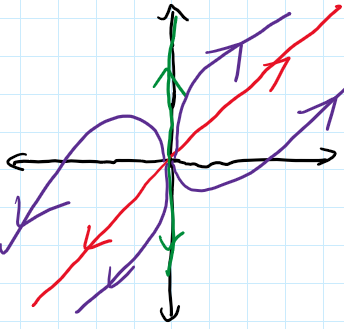
\includegraphics[height=1.5in]{Images/phaseportrait_2_0_1_1_sketch.png}}\hfill\hfill \\
(b) Spiral Sink,\ $C_1e^{-2t}\left[\begin{smallmatrix} -\sin(4t) \\ 2\cos(4t) \end{smallmatrix}\right] + C_2e^{-2t}\left[\begin{smallmatrix} \cos(4t) \\ 2\sin(4t) \end{smallmatrix}\right]$ \hfill\raisebox{-0.5\height}{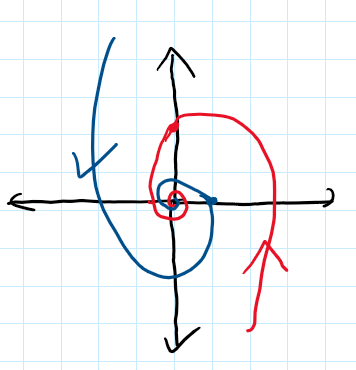
\includegraphics[height=1.5in]{Images/phaseportrait_n2_n2_8_n2_sketch.png}}\hfill\hfill\\
(c) Center,\ $C_1\left[\begin{smallmatrix} 5\cos(4t) \\ -3\cos(4t) = 4\sin(4t) \end{smallmatrix}\right] + C_2 \left[\begin{smallmatrix} 5\sin(4t)\\ 4\cos(4t) - 3\sin(4t) \end{smallmatrix}\right]$ \hfill\raisebox{-0.5\height}{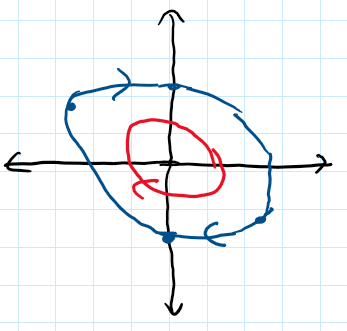
\includegraphics[height=1.5in]{Images/phaseportrait_3_5_n5_n3_sketch.png}}\hfill\hfill\\
(d) Improper Nodal Source,\ $C_1\left[\begin{smallmatrix} 1 \\ 1 \end{smallmatrix}\right]e^{4t} + C_2\left(\left[\begin{smallmatrix} 1 \\ 1  \end{smallmatrix}\right]te^{4t} + \left[\begin{smallmatrix} 1/3 \\ 0 \end{smallmatrix}\right]e^{4t}\right)$ \hfill\raisebox{-0.5\height}{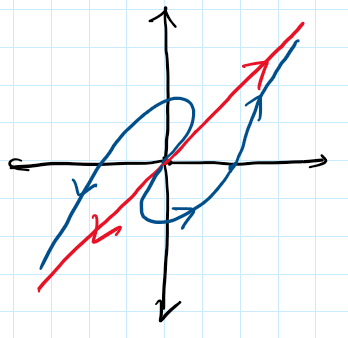
\includegraphics[height=1.5in]{Images/phaseportrait_n1_n3_3_n7_sketch.png}}\hfill\hfill\\
(e) Saddle,\ $C_1\left[\begin{smallmatrix} 1 \\ 0 \end{smallmatrix}\right]e^{3t} + C_2\left[\begin{smallmatrix} 2 \\ -5 \end{smallmatrix}\right]e^{-2t}$ \hfill\raisebox{-0.5\height}{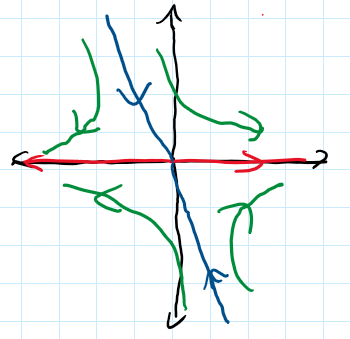
\includegraphics[height=1.5in]{Images/phaseportrait_3_2_0_n2_sketch.png}}\hfill\hfill\\
(f) Spiral Source,\ $C_1e^{3t/2}\left[\begin{smallmatrix} \cos(t/2) \\ \cos(t/2) - \sin(t/2) \end{smallmatrix}\right] + C_2e^{3t/2}\left[\begin{smallmatrix} \sin(t/2) \\ \sin(t/2) + \cos(t/2) \end{smallmatrix}\right]$ \hfill\raisebox{-0.5\height}{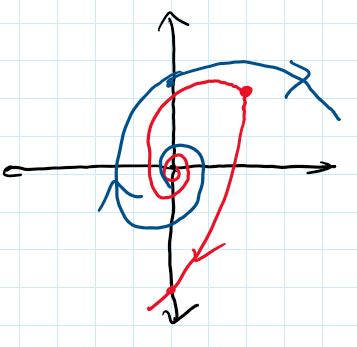
\includegraphics[height=1.5in]{Images/phaseportrait_2_h_n1_1_sketch.png}}\hfill\hfill\\
(g) Saddle,\ $C_1\left[\begin{smallmatrix} 3 \\ 1 \end{smallmatrix}\right]e^{7t/2} + C_2\left[\begin{smallmatrix} -1 \\ 3 \end{smallmatrix}\right]e^{-3t/2}$ \hfill\raisebox{-0.5\height}{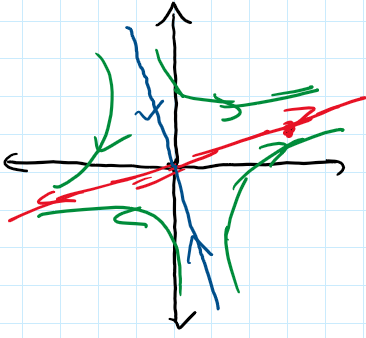
\includegraphics[height=1.5in]{Images/phaseportrait_3_3h_3h_n1_sketch.png}}\hfill\hfill
}%

\begin{exercise}
Consider the second order equation given by
\begin{equation*}
y'' + 2y' - 8y = 0.
\end{equation*}
\begin{tasks}
\task Find the general solution of this problem using the methods of \Chapterref{ho:chapter}.
\task Convert this equation into a first order linear system using the transformation $\vec{x} = \left[ \begin{smallmatrix} y \\ y' \end{smallmatrix} \right]$. 
\task Find the eigenvalues and eigenvalues of the coefficient matrix and use that to find the general solution to the system.
\task Extract the first component of the general solution and compare that to the solution from part (a). How do they relate?
\task Look back through the work. How do the equation used to find the roots in (a) and the eigenvalues in (c) relate to each other?
\end{tasks}
\end{exercise}
\comboSol{%
}
{%
b)~${\vec{x}}' = \left[\begin{smallmatrix} 0 & 1 \\8 & -2 \end{smallmatrix}\right]\vec{x}$ \quad d)~It's the same!
}

\begin{exercise}
Consider the second order equation given by
\begin{equation*}
y'' + 4y' + 5y = 0.
\end{equation*}
\begin{tasks}
\task Find the general solution of this problem using the methods of \Chapterref{ho:chapter}.
\task Convert this equation into a first order linear system using the transformation $\vec{x} = \left[ \begin{smallmatrix} y \\ y' \end{smallmatrix} \right]$. 
\task Find the eigenvalues and eigenvalues of the coefficient matrix and use that to find the general solution to the system.
\task Extract the first component of the general solution and compare that to the solution from part (a). How do they relate?
\task Look back through the work. How do the equation used to find the roots in (a) and the eigenvalues in (c) relate to each other?
\end{tasks}
\end{exercise}
\comboSol{%
}
{%
b)~${\vec{x}}' = \left[\begin{smallmatrix} 0 & 1 \\-4 & -4 \end{smallmatrix}\right]\vec{x}$ \quad d)~It's the same, up to potentially needing to rename the constants ($D_1 = 2C_1 + C_2$ and $D_2 = 2C_2 - C_1$)
}

\begin{exercise}
Consider the second order equation given by
\begin{equation*}
y'' - 4y' + 4y = 0.
\end{equation*} for $b$ and $c$ two real numbers.
\begin{tasks}
\task Find the general solution of this problem using the methods of \Chapterref{ho:chapter}.
\task Convert this equation into a first order linear system using the transformation $\vec{x} = \left[ \begin{smallmatrix} y \\ y' \end{smallmatrix} \right]$. 
\task Find the eigenvalues and eigenvalues of the coefficient matrix and use that to find the general solution to the system.
\task Extract the first component of the general solution and compare that to the solution from part (a). How do they relate?
\task Look back through the work. How do the equation used to find the roots in (a) and the eigenvalues in (c) relate to each other?
\end{tasks}
\end{exercise}
\comboSol{%
}
{%
b)~${\vec{x}}' = \left[\begin{smallmatrix} 0 & 1 \\-4 & 4 \end{smallmatrix}\right]\vec{x}$ \quad d)~It's the same, up to potentially renaming the constants.
}



